\documentclass[]{article}
\usepackage[a4paper, total={6in, 10.5in}]{geometry}
\usepackage[ruled,vlined,linesnumbered]{algorithm2e}
\usepackage{listings}
\usepackage{xcolor}
\usepackage{longtable}
\usepackage{graphicx}

\definecolor{codegreen}{rgb}{0,0.6,0}
\definecolor{codegray}{rgb}{0.5,0.5,0.5}
\definecolor{codepurple}{rgb}{0.58,0,0.82}
\definecolor{backcolour}{rgb}{0.95,0.95,0.92}

\lstdefinestyle{mystyle}{
    backgroundcolor=\color{backcolour},   
    commentstyle=\color{codegreen},
    keywordstyle=\color{magenta},
    numberstyle=\tiny\color{codegray},
    stringstyle=\color{codepurple},
    basicstyle=\ttfamily\footnotesize,
    breakatwhitespace=false,         
    breaklines=true,                 
    captionpos=b,                    
    keepspaces=true,                 
    numbers=left,                    
    numbersep=5pt,                  
    showspaces=false,                
    showstringspaces=false,
    showtabs=false,                  
    tabsize=2,
    frame=single
}

% Title Page
\title{Homework1, Algoritmi su Grafi}
\author{Enrico Cancelli, Alessandro Pegoraro}


\begin{document}
\maketitle

\begin{abstract}
	Una breve relazione sullo svolgimento del progetto. La relazione deve contenere:
	\begin{itemize}
		\item una sezione introduttiva con la descrizione degli algoritmi e delle scelte implementative che avete fatto;
		\item grafici esplicativi dei risultati con le risposte alle due domande;
		\item eventuali originalità introdotte nell'elaborato o nell'implementazione;
		\item una sezione conclusiva in cui porre i vostri commenti e le vostre conclusioni sull'elaborato svolto e i risultati ottenuti
	\end{itemize}
	\textit{/*da eliminare*/}
\end{abstract}

\section{Introduzione}
Lo scopo di questo progetto è l'implementazione e l'analisi di 4 algoritmi di ricerca per il \textit{Minimum Spanning Tree} (in seguito solo MST) di un grafo pesato e non diretto.\\
Questi algoritmi sono:
\begin{itemize}
	\item Algoritmo di Prim
	\item Algoritmo di Kruskal (implementazione naive DFS)
	\item Algoritmo di Kruskal (implementazione naive BFS)
	\item Algoritmo di Kruskal con struttura dati \textit{Union-Find}
\end{itemize}
\subsection{Pseudocodice}
Come riferimento per l'implementazione degli algoritmi è stato preso il seguente pseudo codice spiegato a lezione:\\
\begin{algorithm}[H]
	\SetAlgoLined
	\DontPrintSemicolon
	\KwIn{Graph G}
	\KwIn{vertex s}
	\KwResult{Graph of a MST}
	\For{each u $\in$ V}{
		key[u] $\gets$ +$\infty$\;
		$\pi$[u] $\gets$ NULL\;
	}
	key[s] $\gets$ 0\;
	Q $\gets$ V\;
	\While{Q $\neq$ Ø}{
		u $\gets$ extractMin(Q)\;
		\For{each v adjacent to u}{
			\If{v $\in$ Q and w(u,v) $<$ key[v]}{
				$\pi$[v] $\gets$ u\;
				key[v] $\gets$ w(u,v)\;
			}
		}
	}
	return A\;
	\caption{Prim}
\end{algorithm}

\begin{algorithm}[H]
	\SetAlgoLined
	\DontPrintSemicolon
	\KwIn{Graph G}
	\KwResult{Graph of a MST}
	A = Ø\;
	sort edges of G by cost\;
	\For{each edge e, in nondecreasing order of cost}{
		\If{A $\cup$ {e} is acyclic}{
			A = A $\cup$ {e}\;
		}
	}
	return A\;
	\caption{Kruskal Naive}
\end{algorithm}

\begin{algorithm}[H]
	\SetAlgoLined
	\DontPrintSemicolon
	\KwIn{Graph G}
	\KwResult{Graph of a MST}
	A = Ø\;
	U = initialize(V)\;
	sort edges of E by cost\;
	\For{each edge e=(v,w), in nondecreasing order of cost}{
		\If{Find(U,v) $\neq$ Find(U,w)}{
			A = A $\cup$ {(v,w)}\;
			Union(U,v,w)
		}
	}
	return A\;
	\caption{Kruskal con Union-Find}
\end{algorithm}
\subsection{Struttura del progetto}
Nelle successive sezioni descriveremo in dettaglio l'implementazione di questi algoritmi e delle relative strutture dati di supporto e li testeremo su un dataset generato randomicamente, analizzando i risultati ottenuti e le performance in termini di tempo d'esecuzione e spazio allocato in memoria.\\
I test saranno condotti su grafi non necessariamente semplici (quindi con la possibile presenza di \textit{self loops} e archi multipli tra due nodi) e con pesi non necessariamente positivi.\\
Abbiamo scelto di implementare tali algoritmi utilizzando il linguaggio \textit{C++17} per motivi di efficienza e per potere, allo stesso tempo, utilizzare astrazioni tipiche dei linguaggi ad oggetti rendendo il codice prodotto più modulare.
\section{Implementazione}
In questa sezione verranno esposte e adeguatamente motivate le scelte implementative adottate durante lo sviluppo. L'intero progetto è stato realizzato facendo il più possibile uso di codice generico (template di classe per le strutture dati di supporto e template di funzione per gli algoritmi).\\
Infine verrà data una spiegazione dettagliata sulla struttura del codice realizzato ed eventuali note per la compilazione.
\subsection{Parser}
Considerando che il formato dei grafi di esempio è standardizzato nel seguente modo:
\begin{verbatim}
[numero_di_vertici] [numero_di_archi] 
[un_vertice_arco_1] [altro_vertice_arco_1] [peso_arco_1] 
[un_vertice_arco_2] [altro_vertice_arco_2] [peso_arco_2] 
...
\end{verbatim}
Abbiamo implementato una classe \textbf{Parser} che permette di tradurre solo i file nel formato descritto.\\
Dato che utilizziamo i nodi come indici nelle strutture dati e nei file di esempio i vertici cominciano dall'intero 1, all'interno delle funzioni di parse diminuiamo tutti i nodi di un unità in modo da non sprecare l'indice 0, ciò comunque non porta alcuna differenza alle relazioni tra i nodi e al risultato finale.
\subsection{Strutture dati}
\subsubsection{MinHeap}
\subsubsection{Union-Find}
\subsection{Strutture per la rappresentazione di grafi}
\subsubsection{Edge}
Per rappresentare un lato composto dai  suoi due nodi adiacenti e il peso associato abbiamo creato la classe templetizzata \textbf{Edge$<$W$>$}, con
%TODO tipo del peso non mi piace troppo
\textbf{W} tipo del peso.\\
Nella classe abbiamo ridefinito l'operatore di relazione \textbf{$<$} in modo tale che confronti il peso tra due lati, dato che rappresentiamo l'insieme di lati del grafo \textbf{E} utilizzando un \verb|std::vector|$<$\textbf{Edge}$>$ per poter ordinare i lati in ordine crescente facendo uso della funzione \verb|std::sort()| che prende in input le posizioni estreme del vettore e utilizza l'operatore \textbf{$<$} per l'ordinamento.
\subsubsection{Adjacency List}
Per rappresentare il grafo abbiamo utilizzato una lista di adiacenza implementata dalla classe \textbf{AdjacencyList$<$W$>$}, con \textbf{W} tipo del peso dei lati.\\
La classe è composta da un \verb|std::vector| in cui ogni indice rappresenta un nodo, e ogni elemento è un \verb|std::vector| di coppie \verb|std::pair| nel quale il primo membro è a sua volta un intero che rappresenta un nodo adiacente all'indice, mentre il secondo elemento è il peso associato al lato che collega i due nodi.\\
Nella classe abbiamo implementato \verb|total_weight()| per ottenere il peso totale del grafo, \verb|get_nodes()| e \verb|get_edges()| che ritornano il numero di nodi e di lati.\\
Per verificare se due nodi sono connessi nel grafo abbiamo implementato la funzione ricorsiva \verb|DFS(int v,int w)|:
\lstset{language=c++, style=mystyle}
\lstinputlisting[language=c++]{DFS.cpp}
La quale internamente chiama la funzione privata \verb|DFS_inside(int v, int w, bool L[])| la cui implementazione è la stessa di \verb|DFS| con l'unica differenza che il vettore \verb|L| non è creato ma ricevuto da \verb|DFS|.\\
In \verb|L| ogni indice rappresenta un nodo e ogni elemento indica se quel nodo è stato già visitato durante la ricerca.\\
Abbiamo implementato anche la funzione \verb|BFS(int v,int w)| in forma iterativa per confrontare la velocità tra i due algoritmi in \textbf{Kruskal naive}:
\lstset{language=c++, style=mystyle}
\lstinputlisting[language=c++]{BFS.cpp}
\subsection{Algoritmi}
\subsubsection{Prim}
\newpage
\subsubsection{Naive Kruskal}
\begin{flushleft}
La nostra implementazione presente nel file \verb|algorithms\kruskal_naive.h| è la seguente:

\lstset{language=c++, style=mystyle}
\lstinputlisting[language=c++]{k_naive.cpp}

\textbf{Note implementative:}

\medskip
Per l'ordinamento della lista di lati:

\lstset{language=c++, style=mystyle,backgroundcolor=\color{white}, firstnumber=2}  	 	
\begin{lstlisting}
sort edges of G by cost
\end{lstlisting}

\smallskip
si è utilizzata la funzione \verb|std::sort()| che assicura l'ordinamento in tempo O(non mi ricordo scrivi tu Enrico ammortizzato)%%TODO 
 è stato necessario ridefinire l'operatore booleano di minimo nell'oggetto EDGE
 
\lstset{language=c++, style=mystyle, firstnumber=3} 	 	
\begin{lstlisting}
std::sort(E.begin(), E.end());
\end{lstlisting}

\medskip
Per il controllo dell'aciclicità nel caso di aggiunta di un nuovo lato:

\lstset{language=c++, style=mystyle,backgroundcolor=\color{white}, firstnumber=4}  	 	
\begin{lstlisting}
if A U {e} is acyclic then
\end{lstlisting}

\smallskip
sono stati implementati sia l'algoritmo ricorsivo DFS che l'algoritmo iterativo BFS, queste due funzioni sono state ottimizzate in modo tale che ritornino TRUE solo se esiste un cammino tra i nodi adiacenti al lato che stiamo analizzando.

Se ritornano FALSE allora possiamo aggiungere il nuovo lato alla lista di adiacenza con la certezza che non verrà a formarsi un ciclo.

\lstset{language=c++, style=mystyle, firstnumber=5}
\begin{lstlisting}
if(!A.DFS(E[i].get_node_1(), E[i].get_node_2()))
\end{lstlisting}

\medskip
Inoltre si è ottimizato l'agoritmo con un controllo addizionale per far terminare anticipatamente l'iterazione. 

Viene controllato che il numero di lati non sia mai maggiore o uguale al numero di nodi del grafo.

\lstset{language=c++, style=mystyle, firstnumber=7}
\begin{lstlisting}
if(A.get_edges() == (A.get_nodes() - 1))
    break;
\end{lstlisting}
\end{flushleft}
\subsubsection{Kruskal (con Union-Find)}
\begin{flushleft}
La nostra implementazione presente nel file \verb|algorithms\kruskal_union_find.h| è la seguente:

\lstset{language=c++, style=mystyle}
\lstinputlisting[language=c++]{k_union.cpp}

\textbf{Note implementative:}

\medskip
Per l'inizializzazione della struttura Union-Find:

\lstset{language=c++, style=mystyle,backgroundcolor=\color{white}, firstnumber=2}  	 	
\begin{lstlisting}
U = initialize(V)
\end{lstlisting}

\smallskip
al costruttore è passato un vettore di interi con valori distinti per far si che inizialmente tutti i nodi appartengano a componenti connesse distinte.

\lstset{language=c++, style=mystyle, firstnumber=3}  	 	
\begin{lstlisting}
int *V;
V = new int[n_vec];
std::iota(V, V + n, 0);
UnionFind U(V, n_vec);
\end{lstlisting}

\medskip
Per l'ordinamento della lista di lati:

\lstset{language=c++, style=mystyle,backgroundcolor=\color{white}, firstnumber=2}  	 	
\begin{lstlisting}
sort edges of G by cost
\end{lstlisting}

\smallskip
si è utilizzata la funzione \verb|std::sort()| che assicura l'ordinamento in tempo O(non mi ricordo scrivi tu Enrico ammortizzato)%%TODO 
 è stato necessario ridefinire l'operatore booleano di minimo nell'oggetto EDGE
 
\lstset{language=c++, style=mystyle, firstnumber=7} 	 	
\begin{lstlisting}
std::sort(E.begin(), E.end());
\end{lstlisting}

\medskip
Per controllare se due nodi appartengono alla stessa componente connessa e per unire le componenti connesse
\lstset{language=c++, style=mystyle,backgroundcolor=\color{white}, firstnumber=2}  	 	
\begin{lstlisting}
if Find(U,v) =/= Find(U,w) then
	A = A U (v,w)
	Union(U,v,w)
\end{lstlisting}

\smallskip
sono state implementate le funzioni \verb|U.find()| e \verb|U.unite|.

\lstset{language=c++, style=mystyle, firstnumber=9} 	 	
\begin{lstlisting}
if (U.find(e.get_node_1()) != U.find(e.get_node_2())) {
	A.add(e);
    U.unite(e.get_node_1(), e.get_node_2());
}
\end{lstlisting}

\medskip
Inoltre si è ottimizato l'agoritmo con un controllo addizionale per far terminare anticipatamente l'iterazione. 

Viene controllato che il numero di lati non sia mai maggiore o uguale al numero di nodi del grafo.

\lstset{language=c++, style=mystyle, firstnumber=13}
\begin{lstlisting}
if(A.get_edges() == (A.get_nodes() - 1))
    break;
\end{lstlisting}
\end{flushleft}
\subsection{Note su compilazione e struttura del codice}
\textit{/*forse spostare in sezione a parte?*/}
\section{Testing e analisi sperimentali}
\subsection{Risultati prodotti}
\begin{flushleft}
Di seguito è mostrata la tabella completa dei tempi di esecuzione degli algoritmi per ogni grafo:
\begin{longtable}{|c|c|c|c|c|c|}
\hline
\textbf{GRAPH} & \textbf{PRIM} \textit{(s)} & \textbf{K. UNION-FIND} \textit{(s)} & \textbf{K. DFS} \textit{(s)} & \textbf{K. BFS} \textit{(s)} & \textbf{MST WEIGHT} \\ \hline
1     & 0.0000223 & 0.0000252         & 0.0000118  & 0.0000138  & 29316      \\ \hline
2     & 0.0000219 & 0.0000242         & 0.0000109  & 0.0000151  & 2126       \\ \hline
3     & 0.0000244 & 0.0000264         & 0.0000117  & 0.0000163  & -44765     \\ \hline
4     & 0.0000199 & 0.0000398         & 0.0000114  & 0.0000154  & 20360      \\ \hline
5     & 0.0000454 & 0.0000509         & 0.000021   & 0.0000296  & -32021     \\ \hline
6     & 0.0000428 & 0.0000538         & 0.0000224  & 0.0000336  & 18596      \\ \hline
7     & 0.0000467 & 0.0000559         & 0.0000256  & 0.000037   & -42560     \\ \hline
8     & 0.0000436 & 0.000054          & 0.0000214  & 0.0000318  & -37205     \\ \hline
9     & 0.0000898 & 0.0001214         & 0.0000474  & 0.000068   & -122078    \\ \hline
10    & 0.0000896 & 0.0001185         & 0.0000465  & 0.0000927  & -37021     \\ \hline
11    & 0.0000861 & 0.000116          & 0.0000458  & 0.0000747  & -79570     \\ \hline
12    & 0.0001217 & 0.0001574         & 0.0000648  & 0.0000899  & -79741     \\ \hline
13    & 0.0002631 & 0.0003387         & 0.0001981  & 0.0003148  & -139926    \\ \hline
14    & 0.0002957 & 0.0003759         & 0.0001952  & 0.0003228  & -211345    \\ \hline
15    & 0.0002213 & 0.000322          & 0.0001168  & 0.0001899  & -110571    \\ \hline
16    & 0.0001839 & 0.0002607         & 0.0001468  & 0.0002814  & -233320    \\ \hline
17    & 0.0002809 & 0.0003619         & 0.0001776  & 0.0003533  & -141960    \\ \hline
18    & 0.0002472 & 0.0003346         & 0.0001815  & 0.000301   & -271743    \\ \hline
19    & 0.0003126 & 0.0003215         & 0.0001931  & 0.0002477  & -288906    \\ \hline
20    & 0.0002987 & 0.0003211         & 0.0001544  & 0.0002777  & -232178    \\ \hline
21    & 0.000874  & 0.0009747         & 0.000534   & 0.0009846  & -510185    \\ \hline
22    & 0.0008898 & 0.0013634         & 0.0008088  & 0.0014474  & -515136    \\ \hline
23    & 0.000635  & 0.0009264         & 0.0005399  & 0.0010597  & -444357    \\ \hline
24    & 0.0005683 & 0.0008396         & 0.0006398  & 0.0012851  & -393278    \\ \hline
25    & 0.0015488 & 0.002236          & 0.0029238  & 0.005317   & -1122919   \\ \hline
26    & 0.0010366 & 0.001786          & 0.0017791  & 0.0032735  & -788168    \\ \hline
27    & 0.0014152 & 0.0022047         & 0.0021077  & 0.0047676  & -895704    \\ \hline
28    & 0.0010521 & 0.0017791         & 0.0024222  & 0.0037708  & -733645    \\ \hline
29    & 0.0027576 & 0.0040166         & 0.0109435  & 0.0158155  & -1541291   \\ \hline
30    & 0.0024597 & 0.0042523         & 0.0092917  & 0.014762   & -1578294   \\ \hline
31    & 0.004772  & 0.0050212         & 0.0114346  & 0.018431   & -1675534   \\ \hline
32    & 0.0029573 & 0.0046585         & 0.0158979  & 0.0237307  & -1652119   \\ \hline
33    & 0.0039937 & 0.0060461         & 0.0167154  & 0.0269884  & -2091110   \\ \hline
34    & 0.0068903 & 0.0093624         & 0.0196102  & 0.0359752  & -1934208   \\ \hline
35    & 0.0043936 & 0.0068385         & 0.0257943  & 0.0321756  & -2229428   \\ \hline
36    & 0.0032379 & 0.006222          & 0.0171859  & 0.0347686  & -2359192   \\ \hline
37    & 0.006971  & 0.0118937         & 0.0676218  & 0.0908091  & -4811598   \\ \hline
38    & 0.0052637 & 0.0096671         & 0.0500617  & 0.0815537  & -4739387   \\ \hline
39    & 0.005229  & 0.0093522         & 0.0469542  & 0.0825529  & -4717250   \\ \hline
40    & 0.0052956 & 0.0096173         & 0.046024   & 0.0784298  & -4537267   \\ \hline
41    & 0.0120093 & 0.021044          & 0.213293   & 0.341418   & -8722212   \\ \hline
42    & 0.0109606 & 0.0199926         & 0.190029   & 0.313774   & -9314968   \\ \hline
43    & 0.0105224 & 0.0190362         & 0.177921   & 0.29646    & -9845767   \\ \hline
44    & 0.0104685 & 0.0193646         & 0.194331   & 0.320935   & -8681447   \\ \hline
45    & 0.0224681 & 0.0436783         & 0.796194   & 1.27697    & -17844628  \\ \hline
46    & 0.0217485 & 0.0416504         & 0.791508   & 1.23286    & -18800966  \\ \hline
47    & 0.0243928 & 0.045482          & 0.770846   & 1.34956    & -18741474  \\ \hline
48    & 0.0220459 & 0.0431063         & 0.814875   & 1.31858    & -18190442  \\ \hline
49    & 0.0287203 & 0.0543871         & 1.23424    & 2.03893    & -22086729  \\ \hline
50    & 0.0309194 & 0.0581762         & 1.30569    & 2.04835    & -22338561  \\ \hline
51    & 0.028021  & 0.0538767         & 1.2361     & 1.91129    & -22581384  \\ \hline
52    & 0.0275061 & 0.0541362         & 1.25734    & 1.99845    & -22606313  \\ \hline
53    & 0.0586548 & 0.121006          & 5.20261    & 8.6395     & -45978687  \\ \hline
54    & 0.0594331 & 0.127092          & 5.21449    & 8.25827    & -45195405  \\ \hline
55    & 0.0586596 & 0.123621          & 5.11684    & 8.22975    & -47854708  \\ \hline
56    & 0.0580808 & 0.124887          & 5.14869    & 8.12788    & -46420311  \\ \hline
57    & 0.12261   & 0.272339          & 21.1197    & 33.6028    & -92003321  \\ \hline
58    & 0.122679  & 0.26778           & 21.387     & 34.1273    & -94397064  \\ \hline
59    & 0.12302   & 0.269926          & 20.867     & 33.7653    & -88783643  \\ \hline
60    & 0.122875  & 0.274224          & 21.3095    & 33.4858    & -93017025  \\ \hline
61    & 0.26057   & 0.585217          & 95.386     & 149.296    & -186834082 \\ \hline
62    & 0.261448  & 0.603911          & 95.3925    & 147.101    & -185997521 \\ \hline
63    & 0.260784  & 0.599035          & 95.9979    & 149.658    & -182065015 \\ \hline
64    & 0.266656  & 0.588148          & 92.1425    & 142.189    & -180803872 \\ \hline
65    & 0.341934  & 0.79977           & 165.365    & 255.608    & -230698391 \\ \hline
66    & 0.338952  & 0.772628          & 172.812    & 253.56     & -230168572 \\ \hline
67    & 0.337417  & 0.778169          & 169.326    & 253.897    & -231393935 \\ \hline
68    & 0.341003  & 0.786632          & 166.155    & 252.397    & -231011693 \\ \hline
\caption{\textbf{Tabella riassuntiva dei risultati}}
\end{longtable}
Possiamo osservare come i tempi di esecuzione crescono robe robbe robbbbe robe\\

Medie dei tempi di esecuzione rispetto al numero di nodi:
\begin{longtable}{|c|c|c|c|c|c|}
\hline
\textbf{GRAPH} & \textbf{NODES} & \textbf{PRIM} \textit{(s)} & \textbf{K. UNION-FIND} \textit{(s)} & \textbf{K. DFS} \textit{(s)} & \textbf{K. BFS} \textit{(s)} \\ \hline
1,2,3,4      & 10     & 0.000022125 & 0.0000289     & 0.00001145  & 0.00001515  \\ \hline
5,6,7,8      & 20     & 0.000044625 & 0.00005365    & 0.0000226   & 0.000033    \\ \hline
9,10,11,12      & 40     & 0.0000968   & 0.000128325   & 0.000051125 & 0.000081325 \\ \hline
13,14,15,16      & 80     & 0.000241    & 0.000324325   & 0.000164225 & 0.000277225 \\ \hline
17,18,19,20      & 100    & 0.00028485  & 0.000334775   & 0.00017665  & 0.000294925 \\ \hline
21,22,23,24      & 200    & 0.000741775 & 0.001026025   & 0.000630625 & 0.0011942   \\ \hline
25,26,27,28      & 400    & 0.001263175 & 0.00200145    & 0.0023082   & 0.004282225 \\ \hline
29,30,31,32      & 800    & 0.00323665  & 0.00448715    & 0.011891925 & 0.0181848   \\ \hline
33,34,35,36      & 1000   & 0.004628875 & 0.00711725    & 0.01982645  & 0.03247695  \\ \hline
37,38,39,40      & 2000   & 0.005689825 & 0.010132575   & 0.052665425 & 0.083336375 \\ \hline
41,42,43,44      & 4000   & 0.0109902   & 0.01985935    & 0.1938935   & 0.31814675  \\ \hline
45,46,47,48      & 8000   & 0.022663825 & 0.04347925    & 0.79335575  & 1.2944925   \\ \hline
49,50,51,52      & 10000  & 0.0287917   & 0.05514405    & 1.2583425   & 1.999255    \\ \hline
53,54,55,56      & 20000  & 0.058707075 & 0.1241515     & 5.1706575   & 8.31385     \\ \hline
57,58,59,60      & 40000  & 0.122796    & 0.27106725    & 21.1708     & 33.7453     \\ \hline
61,62,63,64      & 80000  & 0.2623645   & 0.59407775    & 94.729725   & 147.061     \\ \hline
65,66,67,68      & 100000 & 0.3398265   & 0.78429975    & 168.4145    & 253.8655    \\ \hline
\caption{\textbf{Media del tempo di esecuzione rispetto al numero di nodi}}
\end{longtable}

Per ciclare tutto il dataset di grafi (ignorando i tempi per il parsing e contando solo l'esecuzione degli algoritmi):
\begin{longtable}{|c|c|c|c|}
\hline
\textbf{PRIM} \textit{(s)} & \textbf{K. UNION-FIND} \textit{(s)} & \textbf{K. DFS} \textit{(s)} & \textbf{K. BFS} \textit{(s)} \\ \hline
3.449558      & 7.670853               & 1167.276        & 1786.951        \\ \hline  
\caption{\textbf{Tempo di esecuzione totale}}
\end{longtable}
Possiamo osservare come prim e union find sono belli mente DFS e BFS fanno schifo... anche se DFS è un pelino meglio di BFS

\end{flushleft}

\newpage
\subsection{Grafi prodotti}
\begin{flushleft}

Di seguito i grafi dei tempi di esecuzione riferiti ai singoli algoritmi:

\begin{figure}[h]
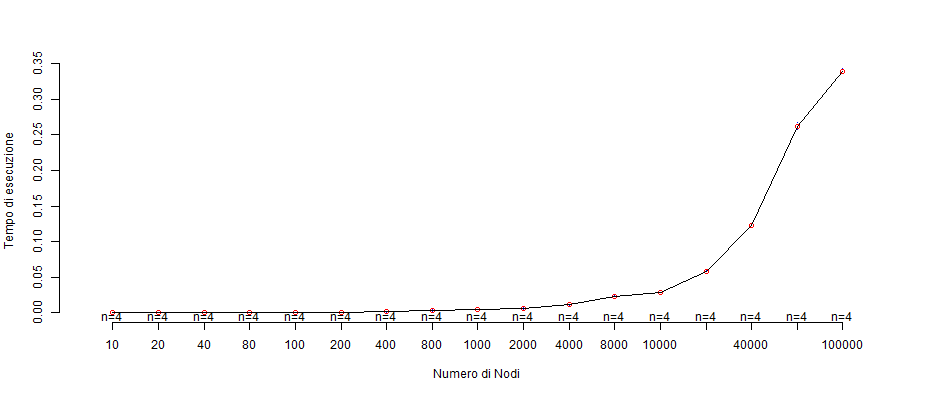
\includegraphics[width=\textwidth,height=\textheight,keepaspectratio]{PRIM_MEDIA.png}
\caption{\textbf{PRIM}}

possiamo osservare che prim fa robe
\end{figure}

\begin{figure}[h]
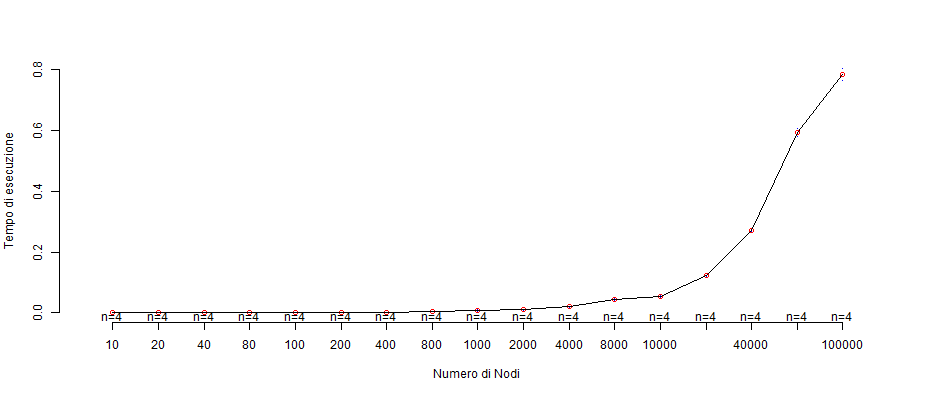
\includegraphics[width=\textwidth,height=\textheight,keepaspectratio]{K_UNION_MEDIA.png}
\caption{\textbf{KRUSKAL UNION-FIND}}

possiamo osservare che union find è leggermente più lento di prim
\end{figure}

\begin{figure}[h]

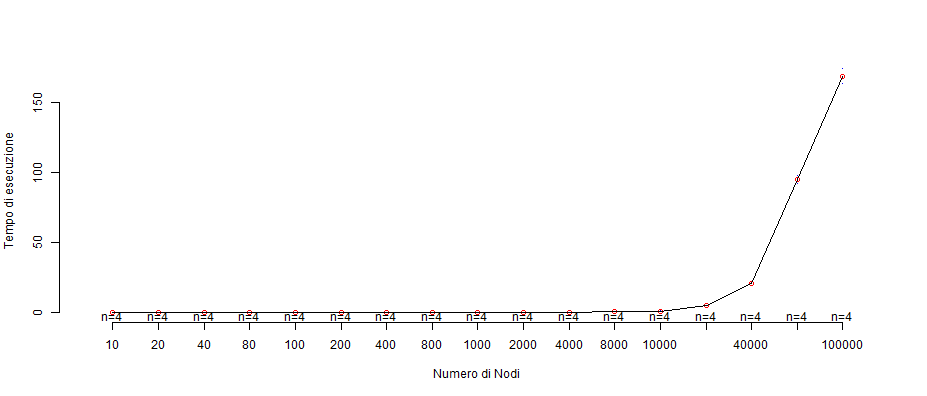
\includegraphics[width=\textwidth,height=\textheight,keepaspectratio]{K_DFS_MEDIA.png}
\caption{\textbf{KRUSKAL DFS}}

possiamo osservare che dfs non è molto buono
\end{figure}

\begin{figure}[h]

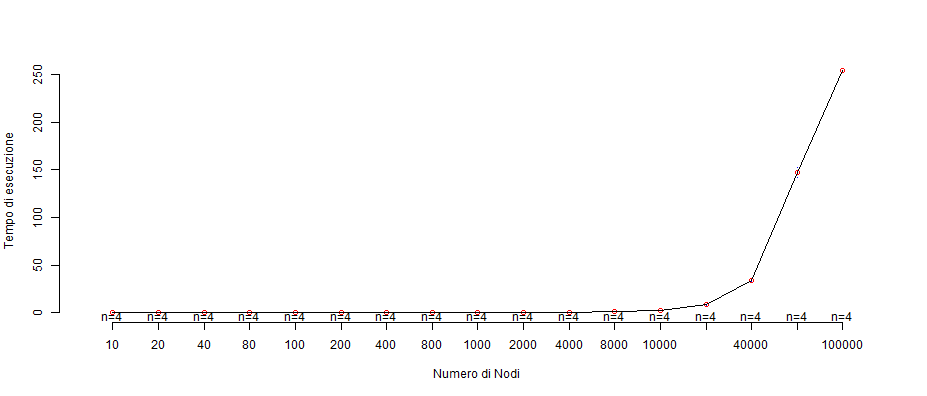
\includegraphics[width=\textwidth,height=\textheight,keepaspectratio]{K_BFS_MEDIA.png}
\caption{\textbf{KRUSKAL BFS}}

possiamo osservare che BFS è il peggiore
\end{figure}

Confrontiamo i due algoritmi migliori e i due algoritmi peggiori:

\begin{figure}[h]

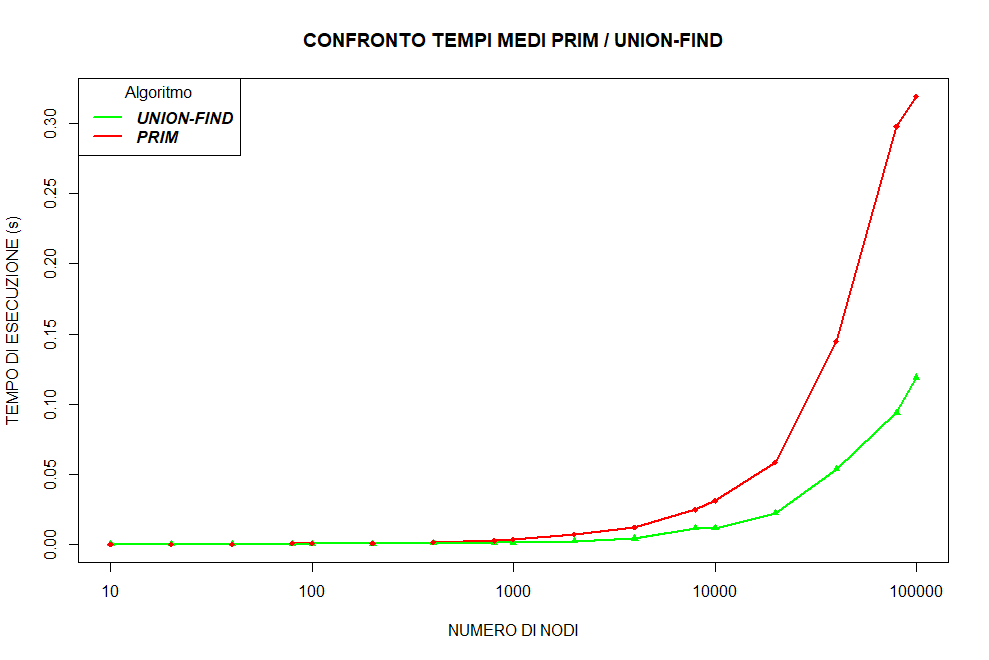
\includegraphics[width=\textwidth,height=\textheight,keepaspectratio]{COMPARE_1.png}
\caption{\textbf{Confronto PRIM e KRUSKAL Union-Find}}

All'inizio i tempi di esecuzione sono molto simili mentre intorno ai 10.000 nodi si inizia a notare una differenza nel tempo di esecuzione
\end{figure}

\begin{figure}[h]

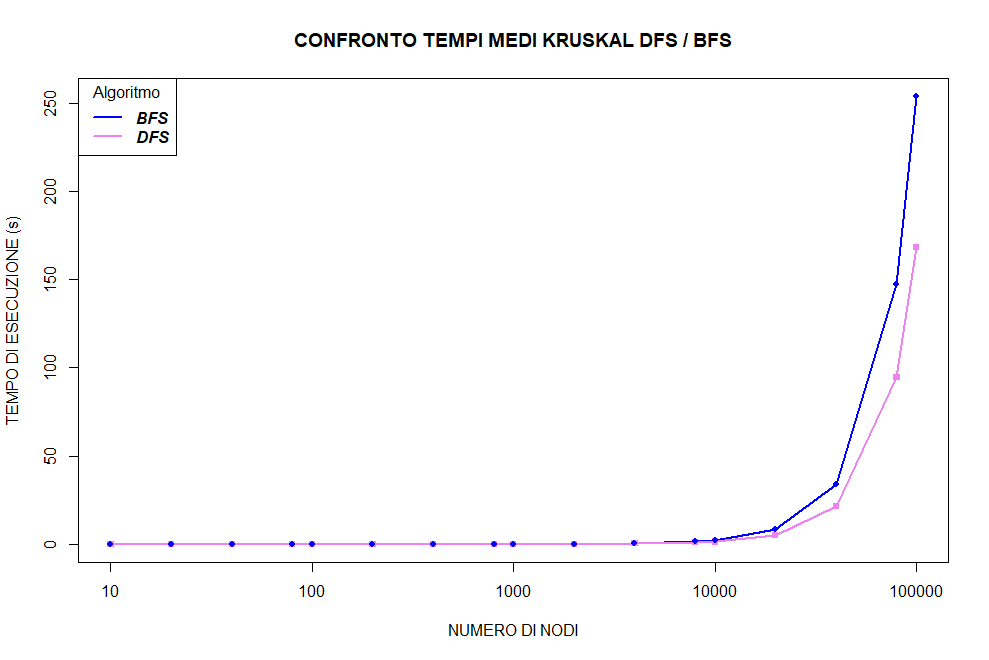
\includegraphics[width=\textwidth,height=\textheight,keepaspectratio]{COMPARE_2.png}
\caption{\textbf{Confronto KRUSKAL DFS e BFS}}

All'inizio i tempi di esecuzione sono molto simili mentre intorno ai 40.000 nodi si inizia a notare una differenza nel tempo di esecuzione
\end{figure}

\end{flushleft}
\newpage
\section{Conclusioni}
\end{document}          
